\documentclass[12pt]{article}
\usepackage[polish]{babel}
\usepackage[T1]{fontenc}
\usepackage[utf8]{inputenc}
\usepackage{float}
\usepackage{graphicx}

\title{\huge\textbf{System zarządzania partią polityczną -- model konceptualny}}
\author{\Large Jakub Grobelny}
\date{\today}

\begin{document}

\maketitle

\section{Diagram E-R}

\begin{figure}[H]
    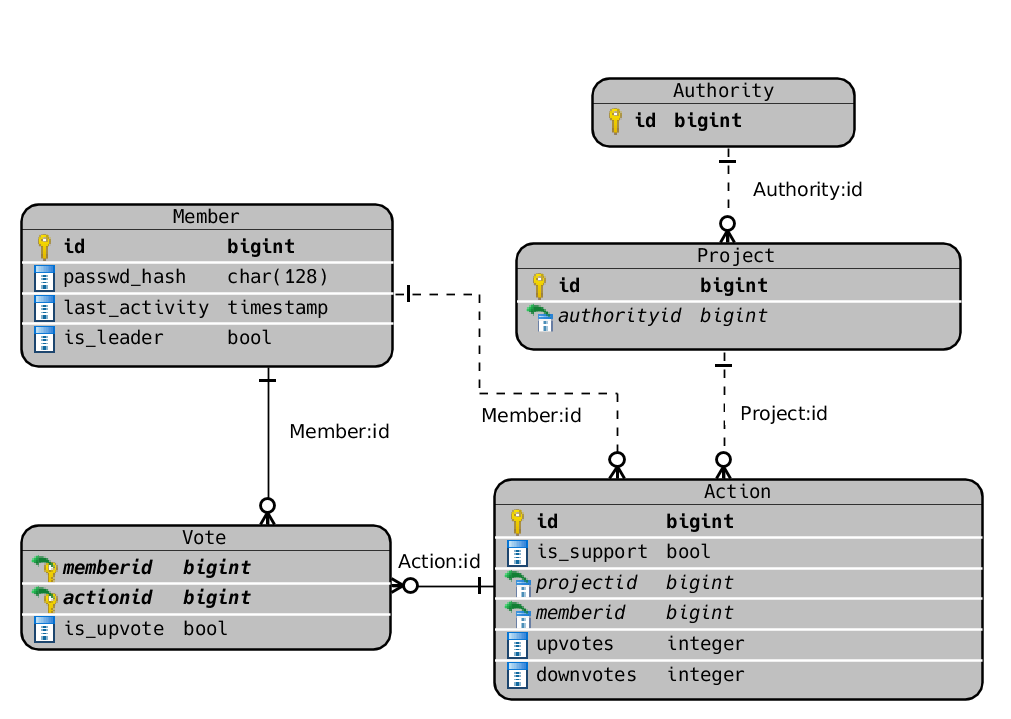
\includegraphics[scale=0.42]{schema.png}
\label{figure:er}
\end{figure}

\section{Opis tabel}

\begin{itemize}
    \item{Tabela \textit{Authority} zawiera spis wszystkich organów władzy
          (przechowywane są jedynie ich identyfikatory.)}
    \item{Tabela \textit{Member} zawiera dane wszystkich członków partii.}
    \begin{itemize}
        \item{\textit{id} -- identyfikator członka.}
        \item{\textit{passwd\char`_hash} -- zahaszowane hasło członka.}
        \item{\textit{last\char`_activity} -- czas ostatniej aktywności członka
              używany w celu stwierdzenia, czy jego konto powinno być zamrożone.}
        \item{\textit{is\char`_leader} -- wartość boolowska prawdziwa jeżeli
              dany członek jest liderem partii. W przeciwnym razie fałsz.}
    \end{itemize}
    \item{Tabela \textit{Project} zawiera wszystkie projekty organizowane
          przez organy władzy.}
    \begin{itemize}
        \item{\textit{id} -- identyfikator projektu.}
        \item{\textit{autorityid} -- identyfikator organu władzy organizującego
              dany projekt. Klucz obcy.}
    \end{itemize}
    \item{Tabela \textit{Action} zawiera wszystkie akcje stworzone przez członków
          partii.}
    \begin{itemize}
        \item{\textit{id} -- identyfikator akcji}
        \item{\textit{is\char`_support} -- wartość boolowska prawdziwa, 
              gdy dana akcjapopiera projekt organu władzy. 
              Fałszywa, gdy akcja jest protestem}
        \item{\textit{projectid} -- identyfikator projektu, którego dotyczy 
              akcja. Klucz obcy.}
        \item{\textit{upvotes} -- liczba wszystkich głosów za daną akcję. Pomaga
              w szybkim wyszukiwaniu \textit{trolli}.}
        \item{\textit{downvotes} -- liczba wszystkich głosów przeciw danej akcji. 
              Pomaga w szybkim wyszukiwaniu \textit{trolli}.}
    \end{itemize}
    \item{Tabela \textit{Vote} zawiera spis wszystkich głosów za i przeciw, 
          które zostały oddane na akcje przez członków partii.}
    \begin{itemize}
        \item{\textit{membeid} -- identyfikator członka, który oddał dany głos.
              Klucz obcy.}
        \item{\textit{actionid} -- identyfikator akcji, na którą oddany został
              dany głos. Klucz obcy.}
        \item{\textit{is\char`_upvote} -- wartość boolowska prawdziwa, gdy dany
              głos jest głosem \textit{za}. Fałsz gdy głos jest \textit{przeciw}.}
    \end{itemize}
\end{itemize}

\section{Użytkownicy}

\begin{itemize}
    \item{}
\end{itemize}

\end{document}


